\documentclass{standalone}
\usepackage{tikz}
\usetikzlibrary{shapes.geometric, arrows.meta, positioning, fit}

\begin{document}
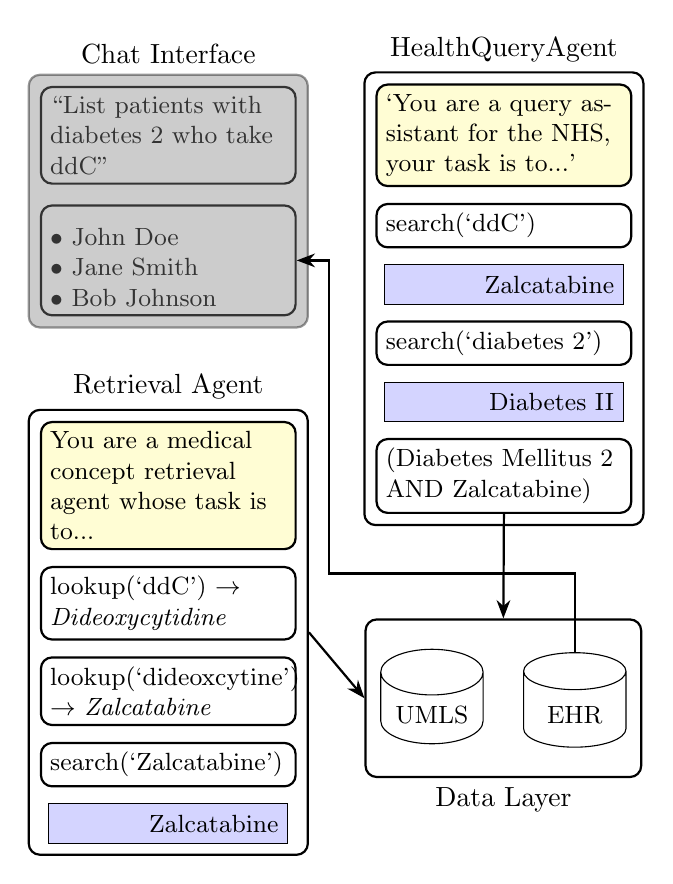
\begin{tikzpicture}[
    node distance=2mm, % vertical spacing between nodes
    innerbox/.style={rectangle, draw, solid, thick, rounded corners, minimum width=1.5cm, minimum height=0.5cm, align=left, text width=3cm, font=\small},
    outerbox/.style={rectangle, draw, thick, rounded corners, minimum width=3.5cm, minimum height=2cm, inner sep=4pt},
    promptbox/.style={innerbox, fill=yellow!17},
    databox/.style={rectangle, draw, solid, minimum width=2.8cm, text width=2.8cm, minimum height=0.5cm, align=left, font=\small, fill=blue!17, align=right},
    arrow/.style={-Stealth, thick},
    data/.style={cylinder, font=\small}
]

% User Interface components
\node[innerbox] (request) {``List patients with diabetes 2 who take ddC''};
\node[innerbox, below=0.25cm of request] (response) {\\$\bullet$ John Doe\\$\bullet$ Jane Smith\\$\bullet$ Bob Johnson};

% Processing components
\node[promptbox, right=1cm of request] (prompt) {`You are a query assistant for the NHS, your task is to...'};
\node[innerbox, below=of prompt] (search1)  {search(`ddC')};
\node[databox, below=of search1] (result1) {Zalcatabine};
\node[innerbox, below=of result1] (search2) {search(`diabetes 2')};
\node[databox, below=of search2] (result2) {Diabetes II};
\node[innerbox, below=of result2] (backend) {(Diabetes Mellitus 2 AND Zalcatabine)};


% Retrieval Sub-agent 
\node[promptbox, below=3cm of request] (retrieval1) {You are a medical concept retrieval agent whose task is to...};
\node[innerbox, below=of retrieval1] (retrieval2) {lookup(`ddC') $\rightarrow$ \textit{Dideoxycytidine}};
\node[innerbox, below=of retrieval2] (retrieval3) {lookup(`dideoxcytine') $\rightarrow$ \textit{Zalcatabine}};
\node[innerbox, below=of retrieval3] (retrieval4) {search(`Zalcatabine')};
\node[databox, below=of retrieval4] (retrieval5) {Zalcatabine};

% Data-Layer
% \node[database, below=3cm of backend] (db) {EHR};
% \node[database, base right=1cm of db.base] (umls) {UMLS};

% Grouping boxes
\node[outerbox, fit=(request) (response), fill=gray, opacity=0.4, label=above:Chat Interface] (interface) {};
\node[outerbox, fit=(prompt) (search1) (result1) (search2) (result2) (backend), label=above:HealthQueryAgent] (processing) {};
\node[outerbox, fit=(retrieval1) (retrieval2) (retrieval3) (retrieval4) (retrieval5), label=above:Retrieval Agent] (retrieval) {};


% Define both database nodes
\node[data, aspect=0.5, draw, shape border rotate=90, minimum height=1.2cm, minimum width=1.3cm, below=1.6cm of processing, xshift=0.9cm] (ehr) {EHR};
\node[data, aspect=0.5, draw, shape border rotate=90, minimum height=1.2cm, minimum width=1.3cm, left=0.5cm of ehr] (umls) {UMLS};

% Then the data layer grouping box that fits both
\node[outerbox, fit=(ehr) (umls), label=below:Data Layer] (data) {};

% Arrows
\draw[arrow] (ehr.north) |- ++(-3.125, 1) |- (response.east);
\draw[arrow] (retrieval.east) -- (data.west);
\draw[arrow] (backend.south) -- (data.north);

% sub-agent dashed-lines
% \draw[dashed] (search1.north west) -- (retrieval.north east);
% \draw[dashed] (result1.south west)  -- (retrieval.south east);

\end{tikzpicture}
\end{document}

